\documentclass[xcolor=dvipsnames]{beamer}

\input{/home/renke/Uni/Formatvorlagen/LaTeX/PackagesPresentations.tex}
\input{/home/renke/Uni/Formatvorlagen/LaTeX/SettingsPresentations.tex}
\hyphenation{li-mi-ting}
\hyphenation{sev-er-al}
\hyphenation{ag-ri-cul-tur-al}

%%% Local Variables:
%%% mode: latex
%%% TeX-master: "../MasArThesis.tex"
%%% End:

\hyphenation{zu-zu-schrei-ben}
\hyphenation{Ge-bie-te}
\hyphenation{Wunsch-er-fül-lung}
\hyphenation{der-ar-ti-ge}
\hyphenation{be-stim-mten}
\hyphenation{be-stim-mte}
\hyphenation{mo-ra-li-sche}
\hyphenation{mo-ra-li-schem}
\hyphenation{mo-ra-li-schen}
\hyphenation{mo-ra-li-scher}
\hyphenation{mo-ra-li-sches}
\hyphenation{Un-rechts-er-eig-nis}
\hyphenation{Rechts-an-sprü-chen}
\hyphenation{Rechts-an-sprü-che}
\hyphenation{Rechts-an-spruch}
\hyphenation{re-le-vant}
\hyphenation{Re-le-vanz}
\hyphenation{Rah-men-be-ding-ung-en}
\hyphenation{fort-ge-setz-ten}
\hyphenation{fort-ge-setzt}
\hyphenation{Ein-tref-fen}
\hyphenation{Ein-tref-fens}
\hyphenation{Le-bens-chan-cen}
\hyphenation{Le-bens-chan-ce}
\hyphenation{mensch-lich-es}
\hyphenation{mensch-lich}
\hyphenation{mensch-lich-er}
\hyphenation{mensch-lich-en}
\hyphenation{Be-schrän-kung}
\hyphenation{Täu-schung}
\hyphenation{be-tref-fen}
\hyphenation{stell-ver-tre-tend}
\hyphenation{Ge-rech-tig-keits-an-sprüche}
\hyphenation{Un-rechts-zu-stand}
\hyphenation{zwi-schen}
\hyphenation{Pflich-ten}
\hyphenation{un-glei-chen}
\hyphenation{mei-nen}
\hyphenation{Eigen-tums-rechts}
\hyphenation{Eigen-tums-recht}
\hyphenation{Rech-ten}
\hyphenation{zu-sätz-li-cher}
\hyphenation{schlech-ten}
\hyphenation{Nicht-i-den-ti-täts-pro-blem}
\hyphenation{Pro-blem}
\hyphenation{zu-kunfts-o-ri-en-tiert}
\hyphenation{be-sei-ti-gen-den}
\hyphenation{Ei-gen-tums-rech-ten}
\hyphenation{Fa-kul-tät}
\hyphenation{For-schungs-an-stal-ten}
\hyphenation{Mo-del-lie-rung}
\hyphenation{Ver-suchs-an-stalt}
\hyphenation{Durch-mes-ser}
\hyphenation{er-trags-kund-licher}
\hyphenation{grund-flä-chen-ge-steu-er-ten}

%%% Local Variables:
%%% mode: latex
%%% TeX-master: "../MasArThesis.tex"
%%% End:


%% Custom commands and environments.
\newcommand{\mycaption}[1]{\tiny\raggedright{#1}}
\newcommand*{\myscalebox}[2][0.6]{\scalebox{#1}{\ensuremath{#2}}}%

%% Define lengths, widths, and heights.
\newlength{\balancedcolumnwidth}
\setlength{\balancedcolumnwidth}{0.49\textwidth}

%% Define slide numbers for managing element visibility.
\newcounter{firstElement}
\newcounter{secondElement}
\newcounter{thirdElement}
\newcounter{fourthElement}
\newcounter{fifthElement}
\newcounter{sixthElement}
\newcounter{seventhElement}
\newcounter{eighthElement}
\newcounter{ninthElement}
\newcounter{tenthElement}
\FPset{\theFirstElement}{1}
\FPadd{\theSecondElement}{\theFirstElement}{1}
\FPadd{\theThirdElement}{\theSecondElement}{1}
\FPadd{\theFourthElement}{\theThirdElement}{1}
\FPadd{\theFifthElement}{\theFourthElement}{1}
\FPadd{\theSixthElement}{\theFifthElement}{1}
\FPadd{\theSeventhElement}{\theSixthElement}{1}
\FPadd{\theEighthElement}{\theSeventhElement}{1}
\FPadd{\theNinthElement}{\theEighthElement}{1}
\FPadd{\theTenthElement}{\theNinthElement}{1}
\FPround{\theSecondElement}{\theSecondElement}{0}
\FPround{\theThirdElement}{\theThirdElement}{0}
\FPround{\theFourthElement}{\theFourthElement}{0}
\FPround{\theFifthElement}{\theFifthElement}{0}
\FPround{\theSixthElement}{\theSixthElement}{0}
\FPround{\theSeventhElement}{\theSeventhElement}{0}
\FPround{\theEighthElement}{\theEighthElement}{0}
\FPround{\theNinthElement}{\theNinthElement}{0}
\FPround{\theTenthElement}{\theTenthElement}{0}

\begin{document}

\title{Modellierung maximaler Grundflächen in gleichaltrigen Reinbeständen}
\subtitle{}
\author{Renke von Seggern}
\date[01.11.2017]{1. November 2017}

\beamertemplatenavigationsymbolsempty

\begin{frame}[plain]
\titlepage
\end{frame}

\addtocounter{framenumber}{-1} %Reduktion der Folienzahl (-1 für Titelfolie)


\section*{}
% \subsubsection*{}
\begin{frame}[c]
  \only<\theFirstElement>{}
\end{frame}

\section{Einleitung}
\subsection{Ziel, Probleme, Lösungsansätze}
\begin{frame}[c]
  \begin{itemize}
  \item<\theFirstElement-> Ziel: \\
    Modellierung der \emph{maximalen} Bestandesgrundfläche in Abhängigkeit von \emph{Alter} und \emph{Bonität} gleichaltriger Buchen- und Fichtenreinbestände
  \item<\theSecondElement-> Probleme:
    \begin{itemize}
    \item<\theSecondElement-> Trainingdatensatz muss von maximalbestockten Flächen stammen
    \item<\theSecondElement-> Direkt messbare Variablen (z.B. \(h_{100}\)) als Prädiktoren ungeeignet, da sie Alters- und Bonitätseffekte enthalten
    \item<\theSecondElement-> Gängige Modelle erscheinen unzureichend
    \end{itemize}
  \end{itemize}
  \begin{itemize}
  \item<\theThirdElement-> Lösungsansätze:
    \begin{itemize}
    \item<\theThirdElement-> Auswahl der Trainingdaten anhand der Mortalitätsrate
    \item<\theThirdElement-> Trennung von Alters- und Bonitätseffekten
    \item<\theThirdElement-> GAM (Generalized Additive Model) und GAMLSS (Generalized Additive Model for Location, Scale and Shape)
    \end{itemize}
  \end{itemize}
\end{frame}

%%% Local Variables:
%%% mode: latex
%%% TeX-master: "MasArPresentation.tex"
%%% End:


\section{Auswahl der Daten}
\subsection{Reineke-Gleichung}
\begin{frame}[c]
  \visible<\theFirstElement->{
    \begin{center}
      \begin{minipage}{0.40\textwidth}
        \centerline{\(\mylog(N) = \textcolor{red}{s} \log(D) + k\)}
        \vspace{\captiondistance}
        \mycaption{Gleichung 1}{Bestandesdichte in Abhängigkeit von mittlerem Durchmesser (Quelle: [1]). \\
          \(N\): Bestandesdichte [\si{\per\hectare}] \\
          \(s\): \textcolor{red}{Steigung} \\
          \(D\): Durchmesser des Grundflächenmittelstammes [\si{\centi\meter}] \\
          \(k\): Konstante (artabhängig)}
      \end{minipage}
    \end{center}

    % \begin{align*}
      % \myscalebox{N} & \myscalebox{: \text{Bestandesdichte [ha\textsuperscript{-1}]}} \\[-3mm]
      % \myscalebox{s} & \myscalebox{: \text{Steigung (}\widehat{=}\text{ \textcolor{red}{Mortalitätsrate})}} \\[-3mm]
      % \myscalebox{D} & \myscalebox{: \text{Durchmesser des Grundflächemittelstammes [cm]}} \\[-3mm]
      % \myscalebox{k} & \myscalebox{: \text{Konstante (artabhängig)}} \\[-3mm]
    % \end{align*}
  }

  \begin{itemize}
  \item<\theSecondElement-> Literatur: \\
    Steigung scheint art- und standortabhängig zu sein (s. z.B. [2])
  \item<\theSecondElement-> Lösungsansatz: \\
    artabhängiger Korridor ,,erlaubter`` Steigungen, begrenzt durch unteren Schwellwert (\(m_u\)) und oberen Schwellwert (\(m_o\))
  \end{itemize}
\end{frame}

\subsection{Auswahlmechanismus}
\begin{frame}[c]
  \begin{columns}
    \begin{column}{0.5\textwidth}
      \visible<\theFirstElement->{
        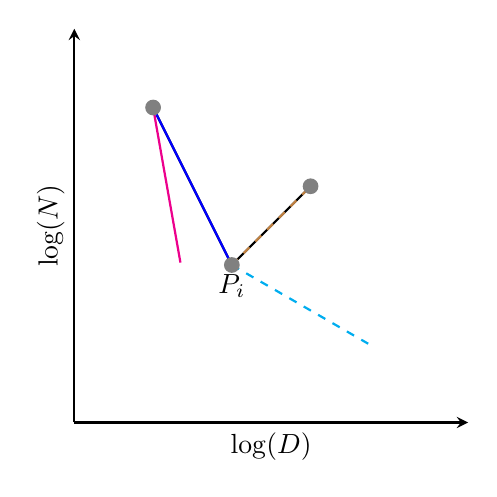
\begin{tikzpicture}[>=stealth]
          %% Coordinate system.
          \draw[black,thick,->] (0,0) -- (5,0);  %% x-axis
          \draw[black,thick,->] (0,0) -- (0,5);  %% y-axis
          \node[anchor=north] at (2.5,0) {\(\log(D)\)};  %% x-axis title
          \node[anchor=south,rotate=90] at (0,2.5) {\(\log(N)\)};  %% y-axis title
          
          %% Specify point coordinates.
          \coordinate (Pi-1) at (1,4);
          \coordinate (Pi) at (2,2);
          \coordinate (Pi+1) at (3,3);

          %% Lines.
          \visible<\theFirstElement-\theSecondElement>{\draw[black,thick] (Pi-1) -- (Pi) -- (Pi+1);}
          \visible<\theSecondElement->{\draw[magenta,thick] (Pi-1) -- ++(280:2cm);}
          \visible<\theSecondElement->{\draw[blue,thick] (Pi-1) -- (Pi);}
          \visible<\theThirdElement->{\draw[cyan,thick,dashed] (Pi) -- ++(330:2cm);}
          \visible<\theThirdElement->{\draw[brown,thick,dashed] (Pi) -- (Pi+1);}

          %% Points.
          \fill[gray] (Pi-1) circle (0.1);
          \fill[gray] (Pi) circle (0.1);
          \fill[gray] (Pi+1) circle (0.1);

          %% Text.
          % \node[anchor=south] at (Pi-1) {\(\text{P}_{i-1}\)};
          \node[anchor=north] at (Pi) {\(\text{P}_i\)};
          % \node[anchor=south] at (Pi+1) {\(\text{P}_{i+1}\)};

        \end{tikzpicture}
        \captionsep{}
        \mycaption{Abbildung 1}{Schematische Darstellung der Funktionsweise des Auswahlmechanismus.}
      }
    \end{column}
    \begin{column}{0.5\textwidth}
      \visible<\theFirstElement->{\(\text{P}_i\) wird ausgewählt, wenn}
      \begin{enumerate}
      \item<\theFirstElement-> es mind. einen benachbarten Punkt gibt (\ding{51}) und
      \item<\theSecondElement-> Steigung \(\textcolor{blue}{s_1} \geq \textcolor{magenta}{m_u}\) (\ding{51}) und
      \item<\theThirdElement-> Steigung \(\textcolor{brown}{s_2} \leq \textcolor{cyan}{m_o}\) (\ding{55}).
      \end{enumerate}
    \end{column}
  \end{columns}
\end{frame}

\subsection{Beispiel: Buche}
\begin{frame}[c]
  \visible<1->{
    \centerline{
      \begin{minipage}{0.9\textwidth}
        \includegraphics[width=1.0\textwidth]{../../Graphics/Presentation/logDlogNPlotsBeforeAfterDataSelectionBeech.pdf}
        \captionsep{}
        \mycaption{Abbildung 2}{Beobachteter Zusammenhang zwischen Bestandesdichte \(N\) und mittlerem Durchmesser \(D\).  Farbige Linien verbinden Beobachtungen eines Bestandes. Gestrichelte bzw. durchgezogene schwarze Linien stellen den oberen bzw. unteren Schwellwert der noch ,,erlaubten`` Steigungen beispielhaft dar. \\
          A: vor Anwendung des Auswahlmechanismus \\
          B: nach Anwendung des Auswahlmechanismus}
      \end{minipage}}}
\end{frame}

%%% Local Variables:
%%% mode: latex
%%% TeX-master: "MasArPresentation.tex"
%%% End:


\addtocounter{framenumber}{-1} %Reduktion der Folienzahl (-1 für Finalfolie)

\section*{}

\begin{frame}[plain]
  \begin{center}
    \setbeamercolor{crane}{fg=letters}
    \setbeamercolor{crane}{bg=boxes}

    \begin{minipage}{0.75\textwidth}
      \begin{beamercolorbox}{crane}
        \begin{center}
          \vspace{1em}
          \textbf{\huge Vielen Dank}
          \\
          \textbf{\small für die Aufmerksamkeit.}
          \\
        \end{center}
      \end{beamercolorbox}
    \end{minipage}

    \hspace{0.017\textwidth}  %% DO NOT change this and the following minipage width, since they were manually set to ensure correct horizontal alignment of the previous and this minipage. 
    \begin{minipage}{0.725\textwidth}
      \setbeamertemplate{enumerate item}{[\insertenumlabel]}
      \begin{block}{Quellen}
        \begin{tiny}
          \begin{enumerate}
          \item \emph{Reineke L. H.} (1933): Perfecting a Stand-Density Index for even-aged Forests. \emph{Journal of Agricultural Research}, 46: 627--638
          \end{enumerate}
        \end{tiny}
      \end{block}
    \end{minipage}
  \end{center}
  
\end{frame}

%%% Local Variables:
%%% mode: latex
%%% TeX-master: "MasArPresentation.tex"
%%% End:


\end{document}

%%% Local Variables:
%%% mode: latex
%%% TeX-master: t
%%% End:
